\section{Generación de señalamiento paso a paso}

Inicialmente, el RNA ejecuta el Algoritmo \ref{alg:graph_network} (ver Sección \ref{sec:grafos}) para detectar todos los \textit{netElements}, sus coordenadas iniciales y finales en la topología, y el sentido en el que fueron definidas. Al concluir el Algoritmo \ref{alg:graph_network}, el RNA ejecuta el Algoritmo \ref{alg:connectedness} (ver Sección \ref{sec:grafos}) para analizar la conexidad de la red. El resultado obtenido se muestra en el Código \ref{lst:EJ4_1}, donde se describen las coordenadas de cada \textit{netElement} y se confirma que la red es conexa.

\begin{lstlisting}[language = {}, tabsize=4, basicstyle=\footnotesize\ttfamily, showspaces=false, showstringspaces=false, caption = Detección de \textit{netElements} por parte del RNA , label = {lst:EJ4_1}]
###### Starting Railway Network Analyzer #####
Reading .railML file
Creating railML object
Analyzing railML object
Analyzing graph
ne991 [-1064, 0] [-2322, 0] <<
ne61 [4350, 0] [4804, 250] >> 
ne63 [4350, 0] [5763, 0] >>
ne65 [7444, 0] [5763, 0] <<
ne910 [11254, 0] [11822, 250] >>
ne912 [11254, 0] [13111, 0] >>
ne114 [15670, 0] [14482, 0] <<
ne288 [-1064, 0] [-741, 250] >>
ne290 [-1064, 0] [-211, 0] >>
ne292 [864, 0] [-211, 0] <<
ne295 [-741, 250] [457, 250] >>
ne297 [457, 250] [720, 250] >>
ne377 [350, -200] [-92, -200] <<
ne384 [457, 250] [-104, 450] <<
ne400 [6904, 250] [7194, 250] >>
ne404 [4804, 250] [6904, 250] >>
ne407 [6904, 250] [5855, 500] <<
ne421 [6454, -259] [5915, -259] <<
ne450 [14722, 250] [14232, 250] <<
ne465 [13772, -259] [13263, -259] <<
ne98 [1573, 0] [3687, 0] >>
ne99 [3687, 0] [4350, 0] >>
ne100 [8372, 0] [10727, 0] >>
ne101 [10727, 0] [11254, 0] >>
ne102 [15670, 0] [18172, 0] >>
ne104 [-509, 630] [-104, 450] >>
ne110 [-104, 450] [-741, 250] <<
ne111 [-211, 0] [-92, -200] >>
ne113 [-92, -200] [-749, -200] <<
ne122 [5304, 759] [5855, 500] >>
ne123 [5855, 500] [4804, 250] <<
ne124 [5763, 0] [5915, -259] >>
ne126 [5915, -259] [5354, -259] <<
ne127 [14232, 250] [13022, 500] <<
ne129 [14232, 250] [14482, 0] >>
ne130 [14232, 250] [11822, 250] <<
ne131 [13111, 0] [13263, -259] >>
ne132 [13111, 0] [14482, 0] >>
ne133 [13263, -259] [12722, -259] <<
ne134 [12452, 810] [13022, 500] >>
ne135 [13022, 500] [11822, 250] <<
ne992 [7444, 0] [8372, 0] >>
ne993 [7194, 250] [7504, 250] >>
ne994 [7444, 0] [7194, 250] <<
ne995 [720, 250] [1020, 250] >>
ne996 [864, 0] [1573, 0] >>
ne997 [720, 250] [864, 0] >>
The network is connected
\end{lstlisting}

Por ejemplo, el \textit{netElement} ne995 inicia en la coordenada (720;250) y finaliza en la coordenada (1020;250). El símbolo $>>$ indica que ne1 se encuentra definido de izquierda a derecha, ya que la componente x de la coordenada final es mayor a la de la coordenada inicial, teniendo la misma componente y. Además, se puede comprobar que la lista obtenida en consistente con la Figura \ref{fig:EJ4_2}. Por ejemplo, ne61, ne63 y ne99 comparten la coordenada (4350;0), que coincide con la coordenada del cambio de vías D05.

A continuación, el RNA detectará la infraestructura ferroviaria, las curvas peligrosas y los puntos medios de los netElements que el RNA considera demasiado largos. El análisis de la infraestructura se detalla en la Sección \ref{sec:bufferstop}, Sección \ref{sec:detectors}, Sección \ref{sec:platform} y Sección \ref{sec:crossing}, mientras que la detección de curvas y puntos medios se detalla en la Sección \ref{sec:tracks}. El RNA ejecuta el Algoritmo \ref{alg:switches_1}, Algoritmo \ref{alg:switches_2} y Algoritmo \ref{alg:switches_3} para confirmar la detección de cambios de vías simples, dobles y en tijeras. El resultado de este proceso se puede visualizar en el Código \ref{lst:EJ4_2}.

\begin{lstlisting}[language = {}, tabsize=4, basicstyle=\footnotesize\ttfamily, showspaces=false, showstringspaces=false, caption = Detección de puntos críticos por parte del RNA , label = {lst:EJ4_2}]
Detecting Danger --> Safe_points.RNA
ne991 has a Middle point @ [-2112.3, 0]
ne991 has a Middle point @ [-1902.7, 0]
ne991 has a Middle point @ [-1693.0, 0]
ne991 has a Middle point @ [-1483.3, 0]
ne991 has a Middle point @ [-1273.7, 0]
ne61 has a Curve(2 lines) @ [[4600, 250]]
ne63 has a Middle point @ [4551.9, 0]
ne63 has a Middle point @ [4753.7, 0]
ne63 has a Middle point @ [4955.6, 0]
ne63 has a Middle point @ [5157.4, 0]
ne63 has a Middle point @ [5359.3, 0]
ne63 has a Middle point @ [5561.1, 0]
ne65 has a Middle point @ [5973.1, 0]
ne65 has a Middle point @ [6183.2, 0]
ne65 has a Middle point @ [6393.4, 0]
ne65 has a Middle point @ [6603.5, 0]
ne65 has a Middle point @ [6813.6, 0]
ne65 has a Middle point @ [7023.8, 0]
ne65 has a Middle point @ [7233.9, 0]
ne910 has a Curve(2 lines) @ [[11504, 250]]
ne912 has a RailJoint[J24] @ [11867, 0]
ne114 has a RailJoint[J27] @ [15294, 0]
ne288 has a Curve(2 lines) @ [[-928, 250]]
ne290 has a RailJoint[J07] @ [-633, 0]
ne292 has a RailJoint[J05] @ [538, 0]
ne295 has a Middle point @ [-501.4, 250]
ne295 has a Middle point @ [-261.8, 250]
ne295 has a Middle point @ [-22.2, 250]
ne295 has a Middle point @ [217.4, 250]
ne297 has a Middle point @ [588.5, 250]
ne377 has a Middle point @ [129.0, -200]
ne384 has a Curve(2 lines) @ [[350, 450]]
ne400 has a Middle point @ [7049.0, 250]
ne404 has a Middle point @ [5014.0, 250]
ne404 has a Middle point @ [5224.0, 250]
ne404 has a Middle point @ [5434.0, 250]
ne404 has a Middle point @ [5644.0, 250]
ne404 has a Middle point @ [5854.0, 250]
ne404 has a Middle point @ [6064.0, 250]
ne404 has a Middle point @ [6274.0, 250]
ne404 has a Middle point @ [6484.0, 250]
ne404 has a Middle point @ [6694.0, 250]
ne407 has a Curve(2 lines) @ [[6654, 500]]
ne421 has a Middle point @ [6184.5, -259]
ne450 has a Middle point @ [14477.0, 250]
ne465 has a Middle point @ [13517.5, -259]
ne98 has a LevelCrossing[lcr495] @ [2419, 0]
ne98 has a LevelCrossing[lcr496] @ [2419, 0]
ne99 has a Middle point @ [3908.0, 0]
ne99 has a Middle point @ [4129.0, 0]
ne100 has a LevelCrossing[lcr497] @ [9346, 0]
ne100 has a LevelCrossing[lcr498] @ [10127, 0]
ne100 has a LevelCrossing[lcr499] @ [9347, 0]
ne100 has a LevelCrossing[lcr500] @ [10127, 0]
ne101 has a RailJoint[J26] @ [10914, 0]
ne102 has a Middle point @ [15878.5, 0]
ne102 has a Middle point @ [16087.0, 0]
ne102 has a Middle point @ [16295.5, 0]
ne102 has a Middle point @ [16504.0, 0]
ne102 has a Middle point @ [16712.5, 0]
ne102 has a Middle point @ [16921.0, 0]
ne102 has a Middle point @ [17129.5, 0]
ne102 has a Middle point @ [17338.0, 0]
ne102 has a Middle point @ [17546.5, 0]
ne102 has a Middle point @ [17755.0, 0]
ne102 has a Middle point @ [17963.5, 0]
ne104 has a Curve(2 lines) @ [[-209, 630]]
ne110 has a Curve(2 lines) @ [[-633, 450]]
ne113 has a Middle point @ [-530.0, -200]
ne113 has a Middle point @ [-311.0, -200]
ne122 has a Curve(2 lines) @ [[5704, 759]]
ne123 has a Curve(2 lines) @ [[5054, 500]]
ne126 has a Middle point @ [5634.5, -259]
ne127 has a Curve(2 lines) @ [[13982, 500]]
ne130 has a Middle point @ [12022.8, 250]
ne130 has a Middle point @ [12223.7, 250]
ne130 has a Middle point @ [12424.5, 250]
ne130 has a Middle point @ [12625.3, 250]
ne130 has a Middle point @ [12826.2, 250]
ne130 has a Middle point @ [13027.0, 250]
ne130 has a Middle point @ [13227.8, 250]
ne130 has a Middle point @ [13428.7, 250]
ne130 has a Middle point @ [13629.5, 250]
ne130 has a Middle point @ [13830.3, 250]
ne130 has a Middle point @ [14031.2, 250]
ne132 has a RailJoint[J21] @ [14309, 0]
ne133 has a Middle point @ [12992.5, -259]
ne134 has a Curve(2 lines) @ [[12842, 810]]
ne135 has a Curve(2 lines) @ [[12072, 500]]
ne992 has a RailJoint[J19] @ [8046, 0]
ne993 has a Middle point @ [7349.0, 250]
ne995 has a Middle point @ [870.0, 250]
ne996 has a RailJoint[J08] @ [1094, 0]
\end{lstlisting}

Esta información es exportada por el RNA, con mayor detalle, en el archivo Infrastructure.RNA (Código \ref{lst:EJ4_4}) que resume cada elemento ferroviario asociado a su respectivo \textit{netElement}.

\begin{lstlisting}[language = {}, tabsize=4, basicstyle=\footnotesize\ttfamily, showspaces=false, showstringspaces=false, caption = Infrastructure.RNA, label = {lst:EJ4_4}]
Nodes: 47|Switches: 23|Signals: 0|Detectors: 8|Ends: 19|Barriers: 2
Node ne991:
	Track = track1
	Type = BufferStop -> ['E16']
	Neighbours = 2 -> ['ne288', 'ne290']
	Switches -> D01
		ContinueCourse -> right -> ne290
		BranchCourse -> left -> ne288
Node ne61:
	Track = track17
	Neighbours = 4 -> ['ne99', 'ne63', 'ne404', 'ne123']
	Switches -> D08
		ContinueCourse -> right -> ne404
		BranchCourse -> left -> ne123
Node ne63:
	Track = track16
	Neighbours = 4 -> ['ne61', 'ne99', 'ne65', 'ne124']
	Switches -> D18
		ContinueCourse -> left -> ne65
		BranchCourse -> right -> ne124
Node ne65:
	Track = track35
	Neighbours = 4 -> ['ne63', 'ne992', 'ne994', 'ne124']
Node ne910:
	Track = track20
	Neighbours = 4 -> ['ne912', 'ne101', 'ne130', 'ne135']
	Switches -> D10
		ContinueCourse -> right -> ne130
		BranchCourse -> left -> ne135
Node ne912:
	Track = track19
	TrainDetectionElements -> tde527
		Type -> insulatedRailJoint
		Side -> left
	Neighbours = 4 -> ['ne910', 'ne101', 'ne131', 'ne132']
	Switches -> D20
		ContinueCourse -> left -> ne132
		BranchCourse -> right -> ne131
Node ne114:
	TrainDetectionElements -> tde534
	Type -> insulatedRailJoint
	Side -> left
	Neighbours = 3 -> ['ne132', 'ne129', 'ne102']
	Switches -> D23
		ContinueCourse -> left -> ne132
		BranchCourse -> right -> ne129
Node ne288:
	Track = track22
	Neighbours = 4 -> ['ne991', 'ne290', 'ne295', 'ne110']
	Switches -> D03
		ContinueCourse -> right -> ne295
		BranchCourse -> left -> ne110
Node ne290:
	Track = track21
	TrainDetectionElements -> tde502
		Type -> insulatedRailJoint
		Side -> left
	Neighbours = 4 -> ['ne991', 'ne288', 'ne292', 'ne111']
	Switches -> D14
		ContinueCourse -> left -> ne292
		BranchCourse -> right -> ne111
Node ne292:
	Track = track33
	TrainDetectionElements -> tde511
		Type -> insulatedRailJoint
		Side -> right
	Neighbours = 4 -> ['ne290', 'ne996', 'ne997', 'ne111']
Node ne295:
	Track = track23
	Neighbours = 4 -> ['ne288', 'ne297', 'ne384', 'ne110']
Node ne297:
	Track = track25
	Neighbours = 4 -> ['ne295', 'ne384', 'ne995', 'ne997']
	Switches -> D04
		ContinueCourse -> left -> ne295
		BranchCourse -> right -> ne384
	Switches -> Sw03
		ContinueCourse -> left -> ne995
		BranchCourse -> right -> ne997
Node ne377:
	Track = track3
	Type = BufferStop -> ['E305']
	Neighbours = 2 -> ['ne111', 'ne113']
	Switches -> D15
		ContinueCourse -> left -> ne113
		BranchCourse -> right -> ne111
Node ne384:
	Track = track26
	Neighbours = 4 -> ['ne295', 'ne297', 'ne104', 'ne110']
Node ne400:
	Track = track27
	Neighbours = 4 -> ['ne404', 'ne407', 'ne993', 'ne994']
	Switches -> D07
		ContinueCourse -> left -> ne404
		BranchCourse -> right -> ne407
	Switches -> Sw02
		ContinueCourse -> left -> ne993
		BranchCourse -> right -> ne994
Node ne404:
	Track = track28
	Neighbours = 4 -> ['ne61', 'ne400', 'ne407', 'ne123']
Node ne407:
	Track = track29
	Neighbours = 4 -> ['ne400', 'ne404', 'ne122', 'ne123']
	Switches -> D16
		ContinueCourse -> left -> ne123
		BranchCourse -> right -> ne122
Node ne421:
	Track = track8
	Type = BufferStop -> ['E418']
	Neighbours = 2 -> ['ne124', 'ne126']
	Switches -> D19
		ContinueCourse -> left -> ne126
		BranchCourse -> right -> ne124
Node ne450:
	Track = track12
	Type = BufferStop -> ['E478']
	Neighbours = 3 -> ['ne127', 'ne129', 'ne130']
Node ne465:
	Track = track10
	Type = BufferStop -> ['E462']
	Neighbours = 2 -> ['ne131', 'ne133']
	Switches -> D21
		ContinueCourse -> left -> ne133
		BranchCourse -> right -> ne131
Node ne98:
	Neighbours = 2 -> ['ne996', 'ne99']
	Level crossing -> Lc01
		Protection -> true | Barriers -> none | Lights -> none Acoustic -> none
		Position -> [2464, 0] | Coordinate: 0.4218
Node ne99:
	Track = track15
	Neighbours = 3 -> ['ne61', 'ne63', 'ne98']
	Switches -> D05
		ContinueCourse -> right -> ne63
		BranchCourse -> left -> ne61
Node ne100:
	Neighbours = 2 -> ['ne992', 'ne101']
	Level crossing -> Lc04
		Protection -> true | Barriers -> none | Lights -> none Acoustic -> none
		Position -> [10172, 0] | Coordinate: 0.7643
Node ne101:
	Track = track18
	TrainDetectionElements -> tde526
		Type -> insulatedRailJoint
		Side -> left
	Neighbours = 3 -> ['ne910', 'ne912', 'ne100']
	Switches -> D09
		ContinueCourse -> right -> ne912
		BranchCourse -> left -> ne910
Node ne102:
	Track = track2
	Type = BufferStop -> ['E109']
	Neighbours = 1 -> ['ne114']
Node ne104:
	Track = track13
	Type = BufferStop -> ['bus541']
	Neighbours = 2 -> ['ne384', 'ne110']
Node ne110:
	Track = track24
	Neighbours = 4 -> ['ne288', 'ne295', 'ne384', 'ne104']
Node ne111:
Track = track34
	Neighbours = 4 -> ['ne290', 'ne292', 'ne377', 'ne113']
Node ne113:
	Track = track5
	Type = BufferStop -> ['E368']
	Neighbours = 2 -> ['ne377', 'ne111']
Node ne122:
	Track = track6
	Type = BufferStop -> ['E408']
	Neighbours = 2 -> ['ne407', 'ne123']
Node ne123:
	Track = track30
	Neighbours = 4 -> ['ne61', 'ne404', 'ne407', 'ne122']
Node ne124:
	Track = track36
	Neighbours = 4 -> ['ne63', 'ne65', 'ne421', 'ne126']
Node ne126:
	Track = track9
	Type = BufferStop -> ['E422']
	Neighbours = 2 -> ['ne421', 'ne124']
Node ne127:
	Track = track39
	Neighbours = 5 -> ['ne450', 'ne129', 'ne130', 'ne135', 'ne134']
	Switches -> D12A
		ContinueCourse -> right -> ne450
		BranchCourse -> left -> ne129
	Switches -> D24
		ContinueCourse -> left -> ne135
		BranchCourse -> right -> ne134
Node ne129:
	Track = track38
	Neighbours = 5 -> ['ne114', 'ne450', 'ne127', 'ne130', 'ne132']
Node ne130:
	Track = track31
	Neighbours = 5 -> ['ne910', 'ne450', 'ne127', 'ne129', 'ne135']
	Switches -> D12B
		ContinueCourse -> right -> ne129
		BranchCourse -> left -> ne450
Node ne131:
	Track = track40
	Neighbours = 4 -> ['ne912', 'ne465', 'ne132', 'ne133']
Node ne132:
	Track = track37
	TrainDetectionElements -> tde533
		Type -> insulatedRailJoint
		Side -> right
	Neighbours = 4 -> ['ne912', 'ne114', 'ne129', 'ne131']
Node ne133:
	Track = track11
	Type = BufferStop -> ['E466']
	Neighbours = 2 -> ['ne465', 'ne131']
Node ne134:
	Track = track14
	Type = BufferStop -> ['bus570']
	Neighbours = 2 -> ['ne127', 'ne135']
Node ne135:
	Track = track32
	Neighbours = 4 -> ['ne910', 'ne127', 'ne130', 'ne134']
Node ne992:	
	TrainDetectionElements -> tde525
		Type -> insulatedRailJoint
		Side -> right
	Neighbours = 3 -> ['ne65', 'ne100', 'ne994']
	Switches -> Sw01
		ContinueCourse -> left -> ne65
		BranchCourse -> right -> ne994
Node ne993:
	Track = track7
	Type = BufferStop -> ['E412']
	Neighbours = 2 -> ['ne400', 'ne994']
Node ne994:
	Track = track41
	Neighbours = 4 -> ['ne65', 'ne400', 'ne992', 'ne993']
Node ne995:
	Track = track4
	Type = BufferStop -> ['E313']
	Neighbours = 2 -> ['ne297', 'ne997']
Node ne996:
	TrainDetectionElements -> tde514
		Type -> insulatedRailJoint
		Side -> right
	Neighbours = 3 -> ['ne292', 'ne98', 'ne997']
	Switches -> Sw04
		ContinueCourse -> left -> ne292
		BranchCourse -> right -> ne997
Node ne997:
	Track = track42
	Neighbours = 4 -> ['ne292', 'ne297', 'ne995', 'ne996']
\end{lstlisting}

	La información de la infraestructura es utilizada por el RNA para detectar los puntos críticos de la red, es decir, las zonas donde es recomendable colocar una señal, según el sentido de circulación que se desee. El resultado es exportado al archivo SafePoints.RNA (Código \ref{lst:EJ4_5}). En el caso de que un mismo \textit{netElement} tenga más de un punto crítico para el mismo sentido, el RNA tomará el más cercano al elemento a proteger. El criterio de selección de puntos críticos se aplica para cada elemento ferroviario detectado, cada curva y cada cambio de vías y fue explicado en las secciones correspondientes ya mencionadas.
	
	\begin{lstlisting}[language = {}, tabsize=4, basicstyle=\footnotesize\ttfamily, showspaces=false, showstringspaces=false, caption = SafePoints.RNA, label = {lst:EJ4_5}]
ne991:
	Next: [[-2112.3, 0], [-1902.7, 0], [-1693.0, 0], [-1483.3, 0], [-1273.7, 0]]
	Prev: [[-2112.3, 0], [-1902.7, 0], [-1693.0, 0], [-1483.3, 0], [-1273.7, 0]]
ne61:
	Prev: [[4700.0, 250]]
ne63:
	Next: [[4551.9, 0], [4753.7, 0], [4955.6, 0], [5157.4, 0], [5359.3, 0], [5561.1, 0]]
	Prev: [[4551.9, 0], [4753.7, 0], [4955.6, 0], [5157.4, 0], [5359.3, 0], [5561.1, 0]]
ne65:
	Next: [[5973.1, 0], [6183.2, 0], [6393.4, 0], [6603.5, 0], [6813.6, 0], [7023.8, 0], [7233.9, 0]]
	Prev: [[5973.1, 0], [6183.2, 0], [6393.4, 0], [6603.5, 0], [6813.6, 0], [7023.8, 0], [7233.9, 0]]
ne910:
	Prev: [[11604.0, 250]]
ne912:
	Next: [[11767.0, 0]]
	Prev: [[11967.0, 0]]
ne114:
	Next: [[15194.0, 0]]
	Prev: [[15394.0, 0]]
ne288:
	Prev: [[-828.0, 250]]
ne290:
	Next: [[-733.0, 0]]
	Prev: [[-533.0, 0]]
ne292:
	Next: [[438.0, 0]]
	Prev: [[638.0, 0]]
ne295:
	Next: [[-501.4, 250], [-261.8, 250], [-22.2, 250], [217.4, 250]]
	Prev: [[-501.4, 250], [-261.8, 250], [-22.2, 250], [217.4, 250]]
ne297:
	Next: [[588.5, 250]]
	Prev: [[588.5, 250]]
ne377:
	Next: [[129.0, -200]]
	Prev: [[129.0, -200]]
ne384:
	Next: [[250.0, 450]]
ne400:
	Next: [[7049.0, 250]]
	Prev: [[7049.0, 250]]
ne404:
	Next: [[5014.0, 250], [5224.0, 250], [5434.0, 250], [5644.0, 250], [5854.0, 250], [6064.0, 250], [6274.0, 250], [6484.0, 250], [6694.0, 250]]
	Prev: [[5014.0, 250], [5224.0, 250], [5434.0, 250], [5644.0, 250], [5854.0, 250], [6064.0, 250], [6274.0, 250], [6484.0, 250], [6694.0, 250]]
ne407:
	Next: [[6554.0, 500]]
ne421:
	Next: [[6184.5, -259]]
	Prev: [[6184.5, -259]]
ne450:
	Next: [[14477.0, 250]]
	Prev: [[14477.0, 250]]
ne465:
	Next: [[13517.5, -259]]
	Prev: [[13517.5, -259]]
ne98:
	Next: [[2219, 0]]
	Prev: [[2619, 0]]
ne99:
	Next: [[3908.0, 0], [4129.0, 0]]
	Prev: [[3908.0, 0], [4129.0, 0]]
ne100:
	Next: [[9927, 0]]
	Prev: [[10327, 0]]
ne101:
	Next: [[10814.0, 0]]
	Prev: [[11014.0, 0]]
ne102:
	Next: [[15878.5, 0], [16087.0, 0], [16295.5, 0], [16504.0, 0], [16712.5, 0], [16921.0, 0], [17129.5, 0], [17338.0, 0], [17546.5, 0], [17755.0, 0], [17963.5, 0]]
	Prev: [[15878.5, 0], [16087.0, 0], [16295.5, 0], [16504.0, 0], [16712.5, 0], [16921.0, 0], [17129.5, 0], [17338.0, 0], [17546.5, 0], [17755.0, 0], [17963.5, 0]]
ne104:
	Next: [[-309.0, 630]]
ne110:
	Prev: [[-533.0, 450]]
ne113:
	Next: [[-530.0, -200], [-311.0, -200]]
	Prev: [[-530.0, -200], [-311.0, -200]]
ne122:
	Next: [[5604.0, 759]]
ne123:
	Prev: [[5154.0, 500]]
ne126:
	Next: [[5634.5, -259]]
	Prev: [[5634.5, -259]]
ne127:
	Next: [[13882.0, 500]]
ne130:
	Next: [[12022.8, 250], [12223.7, 250], [12424.5, 250], [12625.3, 250], [12826.2, 250], [13027.0, 250], [13227.8, 250], [13428.7, 250], [13629.5, 250], [13830.3, 250], [14031.2, 250]]
	Prev: [[12022.8, 250], [12223.7, 250], [12424.5, 250], [12625.3, 250], [12826.2, 250], [13027.0, 250], [13227.8, 250], [13428.7, 250], [13629.5, 250], [13830.3, 250], [14031.2, 250]]
ne132:
	Next: [[14209.0, 0]]
	Prev: [[14409.0, 0]]
ne133:
	Next: [[12992.5, -259]]
	Prev: [[12992.5, -259]]
ne134:
	Next: [[12742.0, 810]]
ne135:
	Prev: [[12172.0, 500]]
ne992:
	Next: [[7946.0, 0]]
	Prev: [[8146.0, 0]]
ne993:
	Next: [[7349.0, 250]]
	Prev: [[7349.0, 250]]
ne995:
	Next: [[870.0, 250]]
	Prev: [[870.0, 250]]
ne996:
	Next: [[994.0, 0]]
	Prev: [[1194.0, 0]]
	\end{lstlisting}
	
	Una vez que el RNA detectó cada punto crítico de la red ferroviaria, procede a generar el señalamiento. El orden en que se procesan los elementos ferroviarios no impacta en el resultado final, pero para poder describirlo de forma ordenada se iniciará generando el señalamiento para proteger los finales de vías, las junturas entre rieles, las plataformas (explicado en la Sección \ref{sec:sig_platform}), los cruces de vía (explicado en la Sección \ref{sec:sig_levelcrossing}) y los cambios de vías (explicado en la Sección \ref{sec:signal_switches}). Luego se procederá a mostrar el señalamiento completo antes y después de la simplificación de señales (explicado en la Sección \label{sec:simplificacion}). 
	
	Tal cómo se explicó en la Sección \ref{sec:sig_border}, el RNA aplica el Algoritmo \ref{alg:lineBorder} y el Algoritmo \ref{alg:bufferStop} para generar las señales para proteger los finales de vías relativos y absolutos. Estas señales son ilustradas en la Figura \ref{fig:EJ4_3}.
	
	\begin{figure}[H]
		\centering
		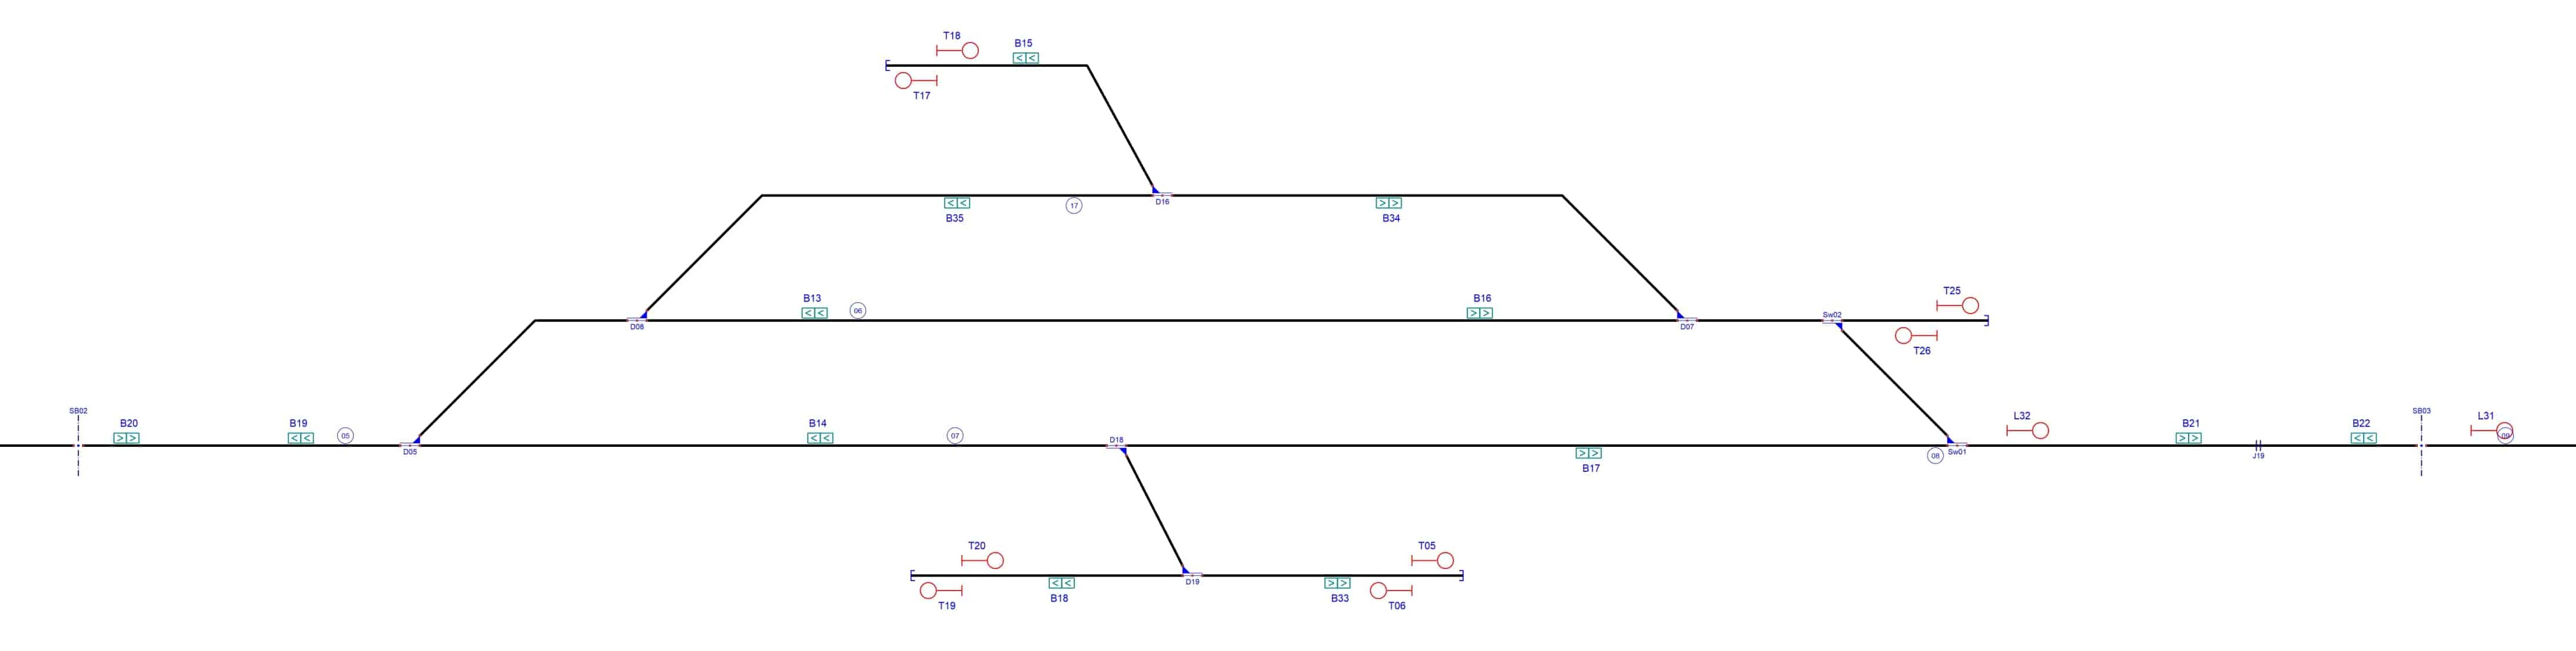
\includegraphics[width=1\textwidth]{resultados-obtenidos/ejemplo4/images/4_step1.png}
		\centering\caption{Señalamiento generado por el RNA para proteger el fin de vía.}
		\label{fig:EJ4_3}
	\end{figure}

	Los finales de vías absolutos son protegidos por las señales de parada T01, T03, T05, T07, T09, T11, T13, T15, T17, T19, T21, T23, T25 y T27; y las señales de partida son T02, T04, T06, T08, T10, T12, T14, T16, T18, T20, T22, T24, T26 y T28. A su vez, al no existir finales de vías relativos, el RNA no les asignó señales específicas.
	
	La Figura \ref{fig:EJ4_4} ilustra la generación de señales destinadas a proteger las junturas entre los rieles. Estas señales se obtuvieron al aplicar el Algoritmo \ref{alg:RJ}, tal como fue explicado en la Sección \ref{sec:sig_joint}. Las señales generadas son todas las señales entre J34 y J49, indicadas en color rojo. De no existir junturas que proteger, el RNA salteará este paso.

	\begin{figure}[H]
		\centering
		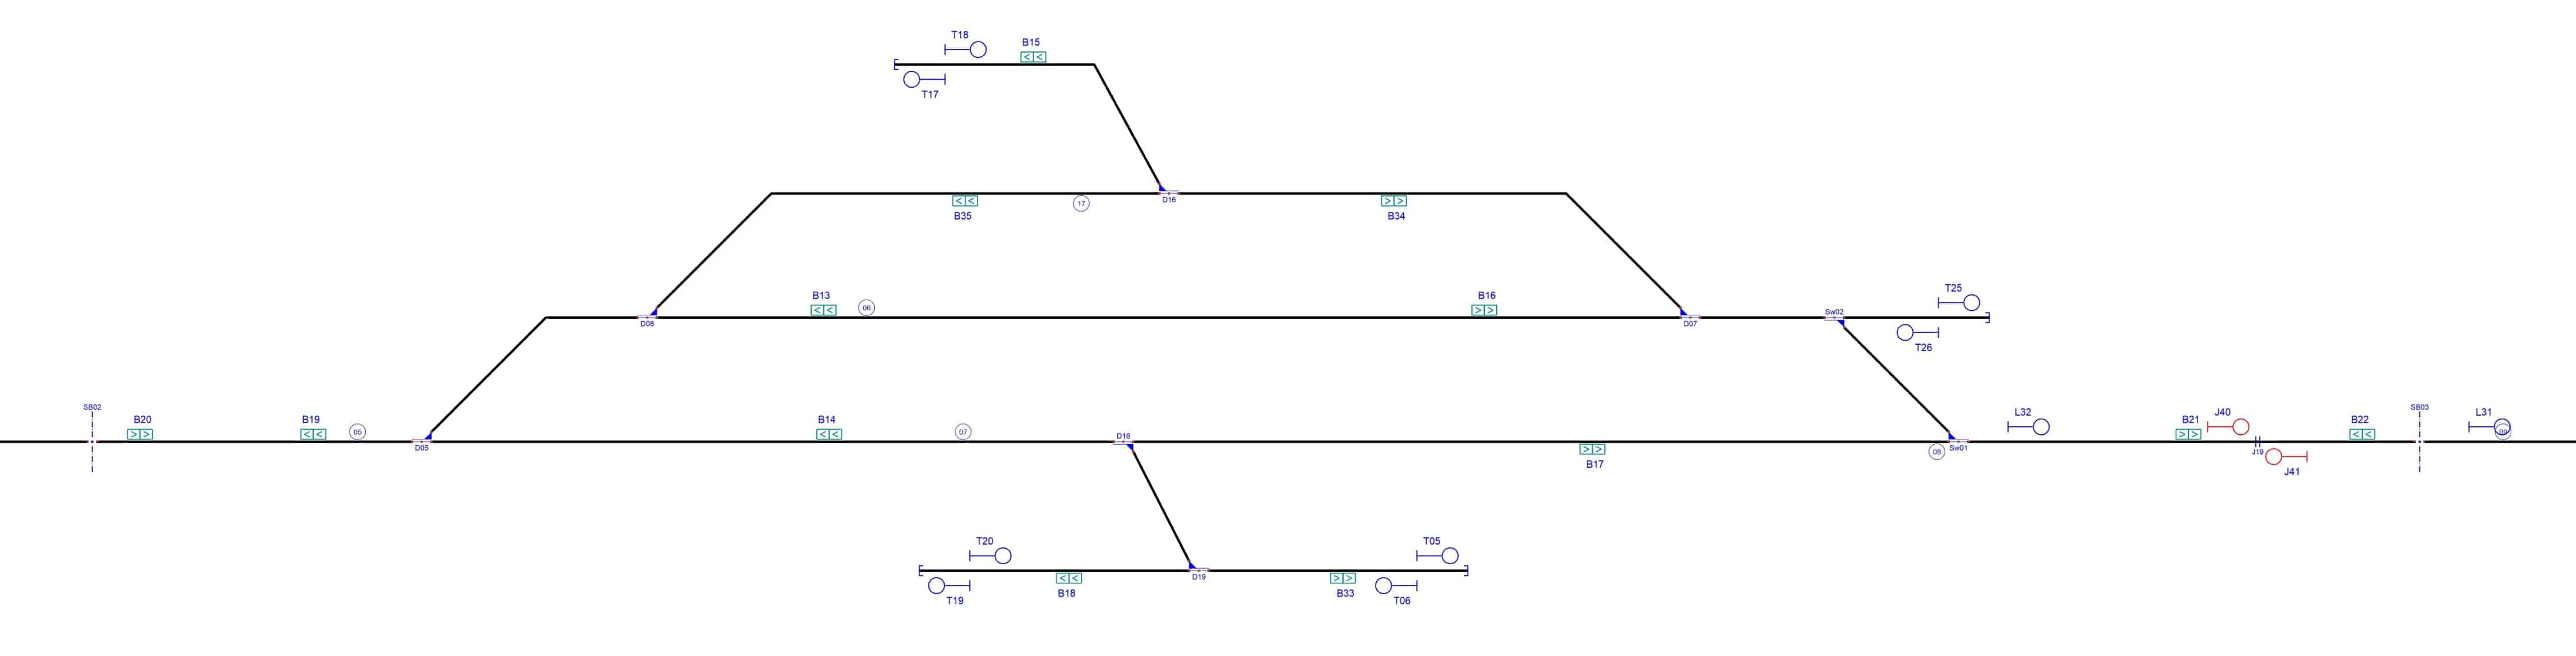
\includegraphics[width=1\textwidth]{resultados-obtenidos/ejemplo4/images/4_step2.png}
		\centering\caption{Señalamiento generado por el RNA para proteger las junturas.}
		\label{fig:EJ4_4}
	\end{figure}

	Al generar el señalamiento para proteger la infraestructura, tal como se explicó en la Sección \ref{sec:horizontal}, el Algoritmo \ref{alg:horizontal} simplificará las señales entre dos elementos ferroviarios si no existe espacio suficiente entre ellos. El señalamiento generado para proteger las plataformas y los cruces de vía, producto de aplicar el Algoritmo \ref{alg:PTF} y el Algoritmo \ref{alg:LC}, respectivamente, se ilustra en rojo en la Figura \ref{fig:EJ1_5}. No se asignaron señales para proteger las plataformas, al no existir en este ejemplo. Por otro lado, las señales que protegen los cruces de vía son las señales comprendidas entre X50 y X53.

	\begin{figure}[H]
		\centering
		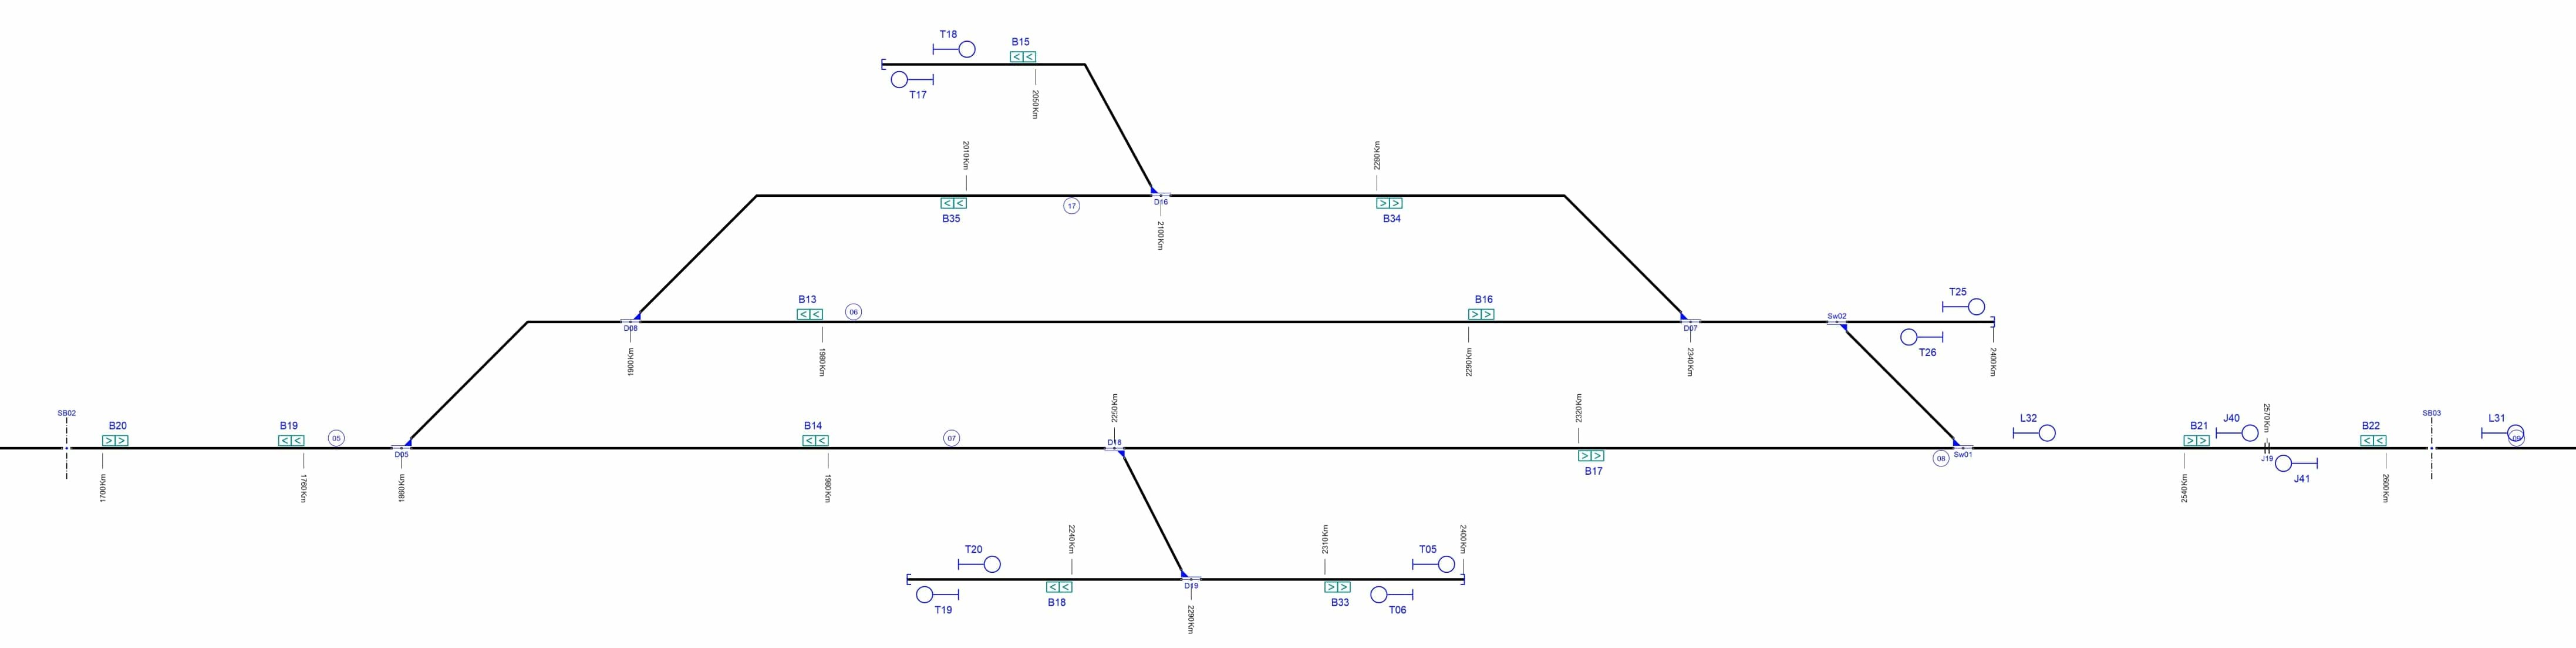
\includegraphics[width=1\textwidth]{resultados-obtenidos/ejemplo4/images/4_step3.png}
		\centering\caption{Señalamiento generado por el RNA para proteger plataformas y cruces de vía.}
		\label{fig:EJ4_5}
	\end{figure}

	Al aplicar el Algoritmo \ref{alg:SW} de generación de señalamiento para cambios de vías, tal como fue explicado en la Sección \label{sec:signal_switches}, el RNA generó 75 señales para proteger cada uno de los cambio de vías. Estas señales se encuentran resaltadas en rojo en la Figura \ref{fig:EJ4_6}.

	\begin{figure}[H]
		\centering
		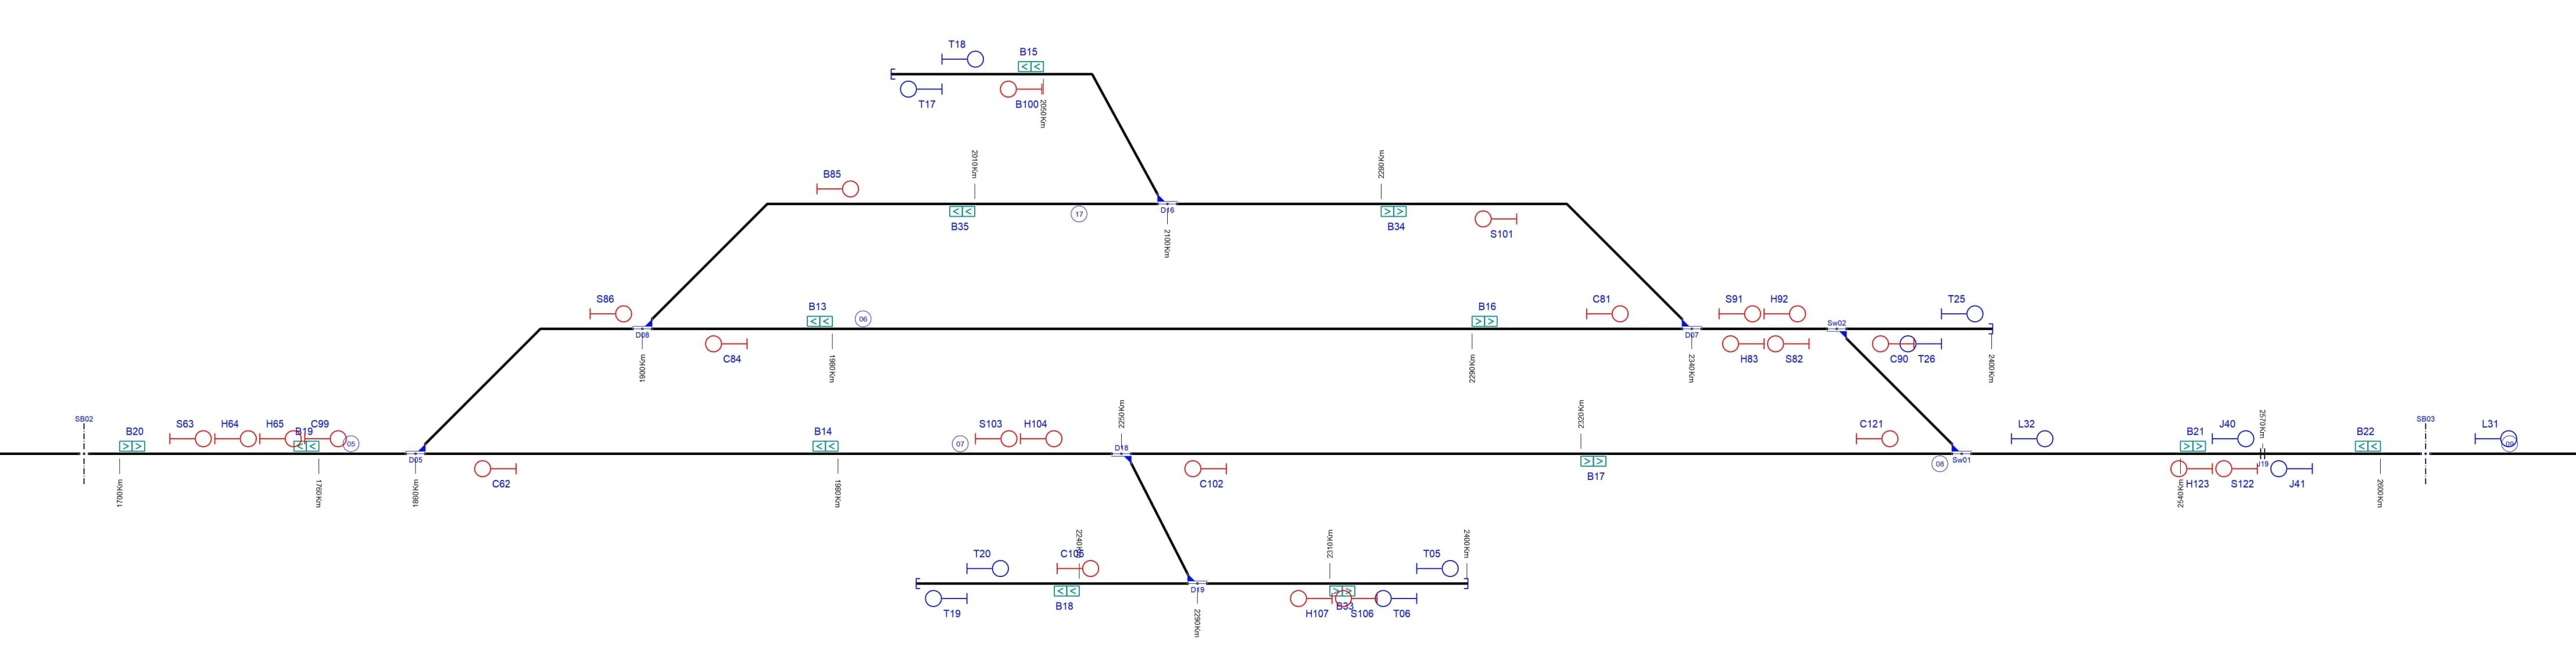
\includegraphics[width=1\textwidth]{resultados-obtenidos/ejemplo4/images/4_step4.png}
		\centering\caption{Señalamiento generado por el RNA para proteger los cambios de vías.}
		\label{fig:EJ4_6}
	\end{figure}

	Una vez obtenido todo el señalamiento, el RNA procede a simplificar las señales redundantes, repetidas o cuyas funciones o ubicaciones se superponen entre sí. El proceso de simplificación de señales fue explicado en la Sección \ref{sec:simplificacion}. El Algoritmo \ref{alg:vertical} de herencia vertical fue aplicado en las señales B entre los cambios de vías que comparan al menos una rama secundaria, desplazando las señales hasta convertirlas en las señales de herencia en las ramas principales. A continuación, se aplicó el Algoritmo \ref{alg:horizontal}, diseñado para agrupar objetos cercanos como un único objeto, generando el señalamiento acorde a los elementos contenidos en cada extremo del nuevo elemento contenedor.
		
	Finalmente, las señales son simplificadas aplicando el Algoritmo \ref{alg:reduction} de eliminación por prioridad de señales. El resultado de este proceso es detallado en el Código \ref{lst:EJ4_3}.

\begin{lstlisting}[language = {}, tabsize=4, basicstyle=\footnotesize\ttfamily, showspaces=false, showstringspaces=false, caption = Reducción de señalamiento por prioridad de señales, label = {lst:EJ4_3}]
	Reducing redundant signals
	removing sig97 for sig04
	removing sig98 for sig04
	removing sig106 for sig06
	removing sig107 for sig06
	removing sig115 for sig10
	removing sig116 for sig10
	removing sig96 for sig16
	removing sig100 for sig17
	removing sig105 for sig20
	removing sig114 for sig22
	removing sig118 for sig23
	removing sig90 for sig26
	removing sig124 for sig28
	removing sig32 for sig40
	removing sig33 for sig38
	removing sig34 for sig94
	removing sig70 for sig35
	removing sig127 for sig36
	removing sig93 for sig37
	removing sig39 for sig128
	removing sig41 for sig122
	removing sig42 for sig67
	removing sig44 for sig112
	removing sig66 for sig45
	removing sig108 for sig46
	removing sig111 for sig47
	removing sig49 for sig109
	removing sig50 for sig52
	removing sig51 for sig53
	removing sig54 for sig58
	removing sig55 for sig59
	removing sig56 for sig60
	removing sig57 for sig61
	removing sig99 for sig63
	removing sig64 for sig63
	removing sig65 for sig63
	removing sig117 for sig67
	removing sig68 for sig67
	removing sig69 for sig67
	removing sig72 for sig71
	removing sig73 for sig71
	removing sig80 for sig79
	removing sig83 for sig82
	removing sig92 for sig91
	removing sig95 for sig94
	removing sig104 for sig103
	removing sig110 for sig109
	removing sig113 for sig112
	removing sig120 for sig119
	removing sig123 for sig122
	removing sig126 for sig125
	removing sig129 for sig128
\end{lstlisting}

	El resultado de la simplificación del señalamiento se ilustra en la Figura \ref{fig:EJ4_7}.
	
	\begin{figure}[H]
		\centering
		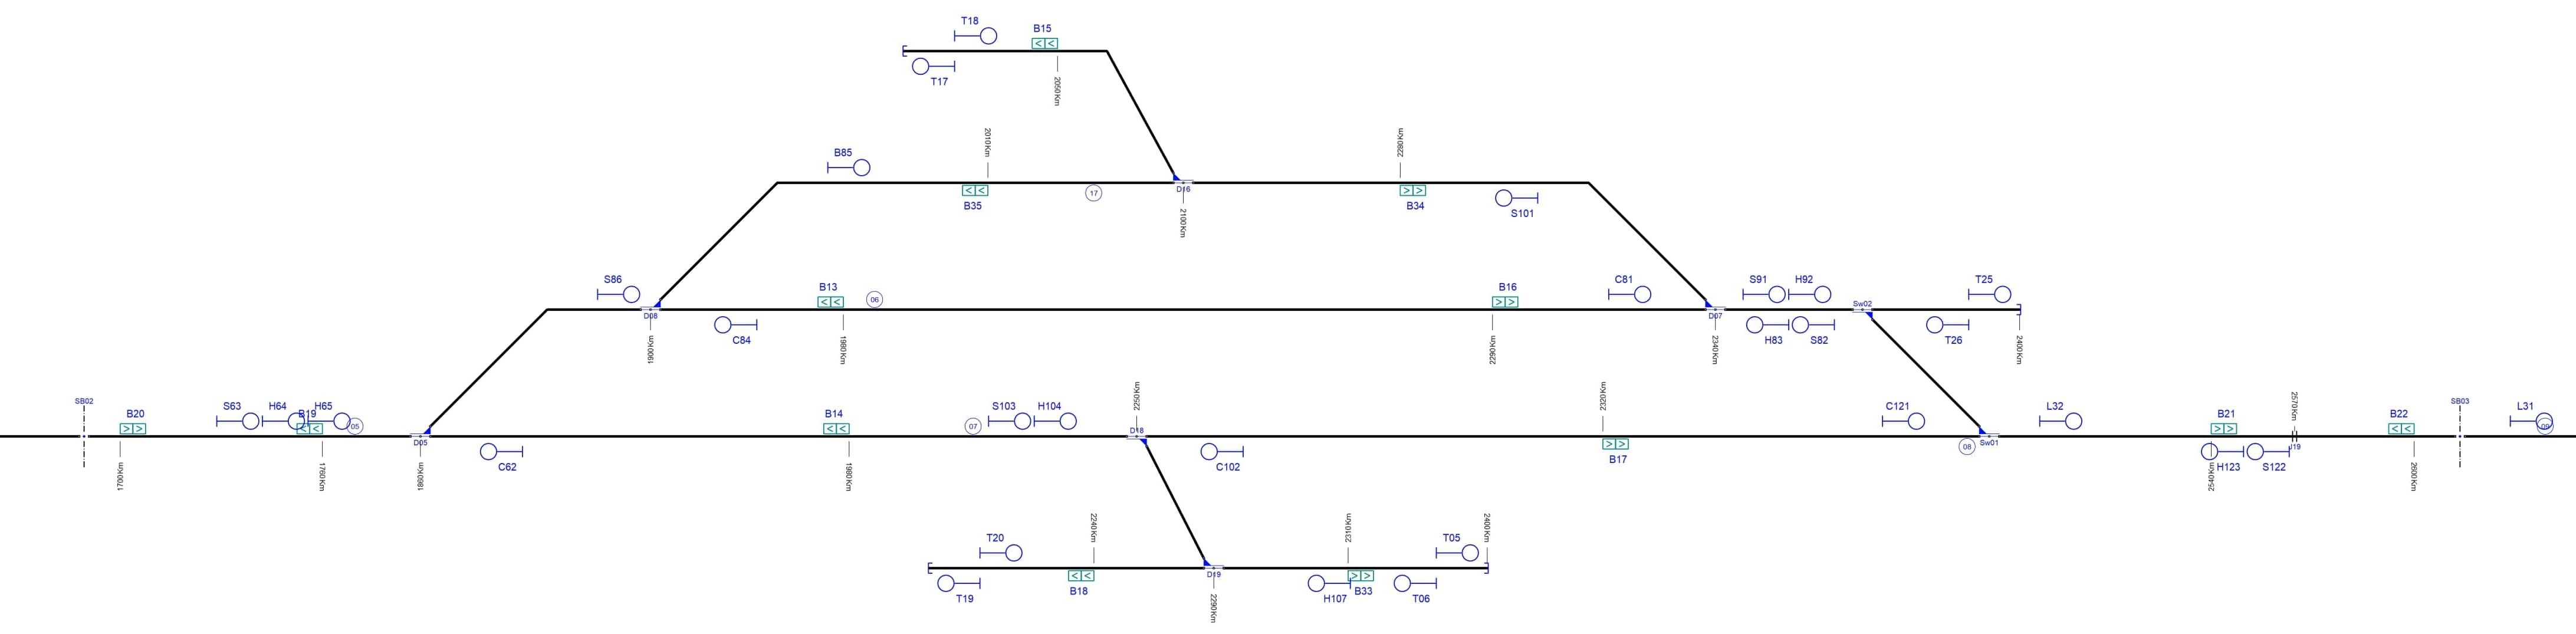
\includegraphics[width=1\textwidth]{resultados-obtenidos/ejemplo4/images/4_RNA.png}
		\centering\caption{Señalamiento generado y simplificado por el RNA.}
		\label{fig:EJ4_7}
	\end{figure}
	
	Además, toda la información del señalamiento generado es exportada por el RNA en el archivo Signalling.RNA (Código \ref{lst:EJ4_6}), que incluye información detallada de la posición, orientación, sentido, coordenada, nombre y tipo de señal.
	
	\begin{lstlisting}[language = {}, tabsize=4, basicstyle=\footnotesize\ttfamily, showspaces=false, showstringspaces=false, caption = Signalling.RNA, label = {lst:EJ4_6}]
T01 [T01] <<:
	From: ne991 | To: E16_left
	Type: Stop | Direction: normal | AtTrack: left 
	Position: [-2222, 0] | Coordinate: 0.0794
T02 [T02] >>:
	From: ne991 | To: ne991_right
	Type: Stop | Direction: reverse | AtTrack: right 
	Position: [-2222, 0] | Coordinate: 0.0794
T03 [T03] >>:
	From: ne377 | To: E305_right
	Type: Stop | Direction: reverse | AtTrack: right 
	Position: [250, 200] | Coordinate: 0.7737
T04 [T04] <<:
	From: ne377 | To: ne377_left
	Type: Stop | Direction: normal | AtTrack: left 
	Position: [250, 200] | Coordinate: 0.7737
T05 [T05] >>:
	From: ne421 | To: E418_right
	Type: Stop | Direction: reverse | AtTrack: right 
	Position: [6354, 259] | Coordinate: 0.8144
T06 [T06] <<:
	From: ne421 | To: ne421_left
	Type: Stop | Direction: normal | AtTrack: left 
	Position: [6354, 259] | Coordinate: 0.8144
T07 [T07] >>:
	From: ne450 | To: E478_right
	Type: Stop | Direction: reverse | AtTrack: right 
	Position: [14622, -250] | Coordinate: 0.7959
T08 [T08] <<:
	From: ne450 | To: ne450_left
	Type: Stop | Direction: normal | AtTrack: left 
	Position: [14622, -250] | Coordinate: 0.7959
T09 [T09] >>:
	From: ne465 | To: E462_right
	Type: Stop | Direction: reverse | AtTrack: right 
	Position: [13672, 259] | Coordinate: 0.8035
T10 [T10] <<:
	From: ne465 | To: ne465_left
	Type: Stop | Direction: normal | AtTrack: left 
	Position: [13672, 259] | Coordinate: 0.8035
T11 [T11] >>:
	From: ne102 | To: E109_right
	Type: Stop | Direction: normal | AtTrack: left 
	Position: [18072, 0] | Coordinate: 0.9600
T12 [T12] <<:
	From: ne102 | To: ne102_left
	Type: Stop | Direction: reverse | AtTrack: right 
	Position: [18072, 0] | Coordinate: 0.9600
T13 [T13] <<:
	From: ne104 | To: bus541_left
	Type: Stop | Direction: reverse | AtTrack: right 
	Position: [-409, -630] | Coordinate: 0.6065
T14 [T14] >>:
	From: ne104 | To: ne104_right
	Type: Stop | Direction: normal | AtTrack: left 
	Position: [-409, -630] | Coordinate: 0.6065
T15 [T15] <<:
	From: ne113 | To: E368_left
	Type: Stop | Direction: normal | AtTrack: left 
	Position: [-649, 200] | Coordinate: 0.1522
T16 [T16] >>:
	From: ne113 | To: ne113_right
	Type: Stop | Direction: reverse | AtTrack: right 
	Position: [-649, 200] | Coordinate: 0.1522
T17 [T17] <<:
	From: ne122 | To: E408_left
	Type: Stop | Direction: reverse | AtTrack: right 
	Position: [5404, -759] | Coordinate: 0.5713
T18 [T18] >>:
	From: ne122 | To: ne122_right
	Type: Stop | Direction: normal | AtTrack: left 
	Position: [5404, -759] | Coordinate: 0.5713
T19 [T19] <<:
	From: ne126 | To: E422_left
	Type: Stop | Direction: normal | AtTrack: left 
	Position: [5454, 259] | Coordinate: 0.1782
T20 [T20] >>:
	From: ne126 | To: ne126_right
	Type: Stop | Direction: reverse | AtTrack: right 
	Position: [5454, 259] | Coordinate: 0.1782
T21 [T21] <<:
	From: ne133 | To: E466_left
	Type: Stop | Direction: normal | AtTrack: left 
	Position: [12822, 259] | Coordinate: 0.1848
T22 [T22] >>:
	From: ne133 | To: ne133_right
	Type: Stop | Direction: reverse | AtTrack: right 
	Position: [12822, 259] | Coordinate: 0.1848
T23 [T23] <<:
	From: ne134 | To: bus570_left
	Type: Stop | Direction: reverse | AtTrack: right 
	Position: [12552, -810] | Coordinate: 0.6125
T24 [T24] >>:
	From: ne134 | To: ne134_right
	Type: Stop | Direction: normal | AtTrack: left 
	Position: [12552, -810] | Coordinate: 0.6125
T25 [T25] >>:
	From: ne993 | To: E412_right
	Type: Stop | Direction: normal | AtTrack: left 
	Position: [7404, -250] | Coordinate: 0.6774
T27 [T27] >>:
	From: ne995 | To: E313_right
	Type: Stop | Direction: normal | AtTrack: left 
	Position: [920, -250] | Coordinate: 0.6666
L29 [L29] >>:
	From: ne114 | To: sb540_left
	Type: Circulation | Direction: reverse | AtTrack: right 
	Position: [14582, 0] | Coordinate: 0.0841
L30 [L30] >>:
	From: ne98 | To: sb537_left
	Type: Circulation | Direction: normal | AtTrack: left 
	Position: [1673, 0] | Coordinate: 0.0473
L31 [L31] >>:
	From: ne100 | To: sb539_left
	Type: Circulation | Direction: normal | AtTrack: left 
	Position: [8472, 0] | Coordinate: 0.0424
J35 [J35] <<:
	From: ne290 | To: ne290_left
	Type: Circulation | Direction: reverse | AtTrack: right 
	Position: [-533.0, 0] | Coordinate: 0.6225
J36 [J36] >>:
	From: ne292 | To: ne292_right
	Type: Circulation | Direction: reverse | AtTrack: right 
	Position: [438.0, 0] | Coordinate: 0.6037
J37 [J37] <<:
	From: ne292 | To: ne292_left
	Type: Circulation | Direction: normal | AtTrack: left 
	Position: [638.0, 0] | Coordinate: 0.7897
J38 [J38] >>:
	From: ne996 | To: ne996_right
	Type: Circulation | Direction: normal | AtTrack: left 
	Position: [994.0, 0] | Coordinate: 0.1833
J40 [J40] >>:
	From: ne992 | To: ne992_right
	Type: Circulation | Direction: normal | AtTrack: left 
	Position: [7946.0, 0] | Coordinate: 0.5409
J43 [J43] <<:
	From: ne101 | To: ne101_left
	Type: Circulation | Direction: reverse | AtTrack: right 
	Position: [11014.0, 0] | Coordinate: 0.5445
J45 [J45] <<:
	From: ne912 | To: ne912_left
	Type: Circulation | Direction: reverse | AtTrack: right 
	Position: [11967.0, 0] | Coordinate: 0.3839
J46 [J46] >>:
	From: ne132 | To: ne132_right
	Type: Circulation | Direction: normal | AtTrack: left 
	Position: [14209.0, 0] | Coordinate: 0.8008
J47 [J47] <<:
	From: ne132 | To: ne132_left
	Type: Circulation | Direction: reverse | AtTrack: right 
	Position: [14409.0, 0] | Coordinate: 0.9467
J48 [J48] >>:
	From: ne114 | To: ne114_right
	Type: Circulation | Direction: reverse | AtTrack: right 
	Position: [15194.0, 0] | Coordinate: 0.5993
X50 [X50] >>:
	From: ne98 | To: ne98_right
	Type: Circulation | Direction: normal | AtTrack: left 
	Position: [2219, 0] | Coordinate: 0.3055
X51 [X51] <<:
	From: ne98 | To: ne98_left
	Type: Circulation | Direction: reverse | AtTrack: right 
	Position: [2619, 0] | Coordinate: 0.4947
X52 [X52] >>:
	From: ne100 | To: ne100_right
	Type: Circulation | Direction: normal | AtTrack: left 
	Position: [9927, 0] | Coordinate: 0.6602
X53 [X53] <<:
	From: ne100 | To: ne100_left
	Type: Circulation | Direction: reverse | AtTrack: right 
	Position: [10327, 0] | Coordinate: 0.8301
C54 [C54] <<:
	From: ne63 | To: ne63_left
	Type: Circulation | Direction: reverse | AtTrack: right 
	Position: [4551.9, 0] | Coordinate: 0.1428
S55 [S55] >>:
	From: ne99 | To: ne99_right
	Type: Circulation | Direction: normal | AtTrack: left 
	Position: [4129.0, 0] | Coordinate: 0.6666
S59 [S59] >>:
	From: ne101 | To: ne101_right
	Type: Circulation | Direction: normal | AtTrack: left 
	Position: [11014.0, 0] | Coordinate: 0.5445
S64 [S64] >>:
	From: ne991 | To: ne991_right
	Type: Circulation | Direction: reverse | AtTrack: right 
	Position: [-1273.7, 0] | Coordinate: 0.8333
C67 [C67] <<:
	From: ne295 | To: ne295_left
	Type: Circulation | Direction: reverse | AtTrack: right 
	Position: [-501.4, -250] | Coordinate: 0.2
B68 [B68] >>:
	From: ne110 | To: ne110_left
	Type: Manouver | Direction: reverse | AtTrack: right 
	Position: [-533.0, -450] | Coordinate: 0.4327
S69 [S69] >>:
	From: ne288 | To: ne288_right
	Type: Circulation | Direction: normal | AtTrack: left 
	Position: [-828.0, -250] | Coordinate: 0.8155
C70 [C70] >>:
	From: ne295 | To: ne295_right
	Type: Circulation | Direction: normal | AtTrack: left 
	Position: [217.4, -250] | Coordinate: 0.7999
B71 [B71] <<:
	From: ne384 | To: ne384_right
	Type: Manouver | Direction: normal | AtTrack: left 
	Position: [250.0, -450] | Coordinate: 0.8531
S72 [S72] <<:
	From: ne297 | To: ne297_left
	Type: Circulation | Direction: reverse | AtTrack: right 
	Position: [588.5, -250] | Coordinate: 0.5
C74 [C74] >>:
	From: ne404 | To: ne404_right
	Type: Circulation | Direction: normal | AtTrack: left 
	Position: [6694.0, -250] | Coordinate: 0.9
S75 [S75] <<:
	From: ne400 | To: ne400_left
	Type: Circulation | Direction: reverse | AtTrack: right 
	Position: [7049.0, -250] | Coordinate: 0.5
C77 [C77] <<:
	From: ne404 | To: ne404_left
	Type: Circulation | Direction: reverse | AtTrack: right 
	Position: [5014.0, -250] | Coordinate: 0.1
B78 [B78] >>:
	From: ne123 | To: ne123_left
	Type: Manouver | Direction: reverse | AtTrack: right 
	Position: [5154.0, -500] | Coordinate: 0.3928
S79 [S79] >>:
	From: ne61 | To: ne61_right
	Type: Circulation | Direction: normal | AtTrack: left 
	Position: [4700.0, -250] | Coordinate: 0.8134
C80 [C80] <<:
	From: ne130 | To: ne130_left
	Type: Circulation | Direction: normal | AtTrack: left 
	Position: [12022.8, -250] | Coordinate: 0.0833
B81 [B81] >>:
	From: ne135 | To: ne135_left
	Type: Manouver | Direction: reverse | AtTrack: right 
	Position: [12172.0, -500] | Coordinate: 0.3479
S82 [S82] >>:
	From: ne910 | To: ne910_right
	Type: Circulation | Direction: normal | AtTrack: left 
	Position: [11604.0, -250] | Coordinate: 0.6753
C83 [C83] <<:
	From: ne993 | To: ne993_left
	Type: Circulation | Direction: reverse | AtTrack: right 
	Position: [7349.0, -250] | Coordinate: 0.5
S84 [S84] >>:
	From: ne400 | To: ne400_right
	Type: Circulation | Direction: normal | AtTrack: left 
	Position: [7049.0, -250] | Coordinate: 0.5
S87 [S87] >>:
	From: ne290 | To: ne290_right
	Type: Circulation | Direction: normal | AtTrack: left 
	Position: [-533.0, 0] | Coordinate: 0.6225
S94 [S94] <<:
	From: ne407 | To: ne407_left
	Type: Circulation | Direction: normal | AtTrack: left 
	Position: [6554.0, -500] | Coordinate: 0.9132
C95 [C95] <<:
	From: ne65 | To: ne65_left
	Type: Circulation | Direction: normal | AtTrack: left 
	Position: [5973.1, 0] | Coordinate: 0.1249
S96 [S96] >>:
	From: ne63 | To: ne63_right
	Type: Circulation | Direction: normal | AtTrack: left 
	Position: [5561.1, 0] | Coordinate: 0.8571
S102 [S102] <<:
	From: ne114 | To: ne114_left
	Type: Circulation | Direction: normal | AtTrack: left 
	Position: [15194.0, 0] | Coordinate: 0.5993
S105 [S105] >>:
	From: ne127 | To: ne127_right
	Type: Circulation | Direction: reverse | AtTrack: right 
	Position: [13882.0, -500] | Coordinate: 0.9238
S108 [S108] >>:
	From: ne130 | To: ne130_right
	Type: Circulation | Direction: reverse | AtTrack: right 
	Position: [14031.2, -250] | Coordinate: 0.9166
S111 [S111] >>:
	From: ne912 | To: ne912_right
	Type: Circulation | Direction: normal | AtTrack: left 
	Position: [11967.0, 0] | Coordinate: 0.3839
S118 [S118] <<:
	From: ne127 | To: ne127_left
	Type: Circulation | Direction: normal | AtTrack: left 
	Position: [13882.0, -500] | Coordinate: 0.9238
C120 [C120] >>:
	From: ne65 | To: ne65_right
	Type: Circulation | Direction: reverse | AtTrack: right 
	Position: [7233.9, 0] | Coordinate: 0.8750
S121 [S121] <<:
	From: ne992 | To: ne992_left
	Type: Circulation | Direction: reverse | AtTrack: right 
	Position: [7946.0, 0] | Coordinate: 0.5409
C123 [C123] <<:
	From: ne995 | To: ne995_left
	Type: Circulation | Direction: reverse | AtTrack: right 
	Position: [870.0, -250] | Coordinate: 0.5
S124 [S124] >>:
	From: ne297 | To: ne297_right
	Type: Circulation | Direction: normal | AtTrack: left 
	Position: [588.5, -250] | Coordinate: 0.5
S127 [S127] <<:
	From: ne996 | To: ne996_left
	Type: Circulation | Direction: reverse | AtTrack: right 
	Position: [994.0, 0] | Coordinate: 0.1833
	\end{lstlisting}	
	
	Al finalizar la generación del señalamiento, el RNA ejecuta el Algoritmo \ref{alg:routes}, explicado en la Sección \ref{sec:rutas}, para detectar todas las posibles rutas admitidas por la red para crear la tabla de enclavamientos. La cuál puede ser visualizada en el archivo Routes.RNA (Código \ref{lst:EJ4_7}). La misma detalla las señales de inicio y final, los \textit{netElements} abarcados por la ruta y cualquier infraestructura involucrada, incluyendo el estado que deben tener para que la ruta sea activada.
	
	\begin{lstlisting}[language = {}, tabsize=4, basicstyle=\footnotesize\ttfamily, showspaces=false, showstringspaces=false, caption = Routes.RNA, label = {lst:EJ4_7}]
route_1 [T02 >> S64]:
	Path: ['ne991']
route_2 [T04 << J35]:
	Path: ['ne377', 'ne111', 'ne290']
	Switches: ['D14_R', 'D15_R']
route_3 [T04 << T15]:
	Path: ['ne377', 'ne113']
	Switches: ['D15_N']
route_4 [T06 << C54]:
	Path: ['ne421', 'ne124', 'ne63']
	Switches: ['D18_R', 'D19_R']
route_5 [T06 << T19]:
	Path: ['ne421', 'ne126']
	Switches: ['D19_N']
route_6 [T08 << S118]:
	Path: ['ne450', 'ne127']
	Switches: ['D12_RN']
route_7 [T08 << C80]:
	Path: ['ne450', 'ne130']
	Switches: ['D12_NN']
route_8 [T10 << J45]:
	Path: ['ne465', 'ne131', 'ne912']
	Switches: ['D20_R', 'D21_R']
route_9 [T10 << T21]:
	Path: ['ne465', 'ne133']
	Switches: ['D21_N']
route_10 [T12 << S102]:
	Path: ['ne102', 'ne114']
route_11 [T14 >> S124]:
	Path: ['ne104', 'ne384', 'ne297']
	Switches: ['D04_R']
route_12 [T16 >> T03]:
	Path: ['ne113', 'ne377']
	Switches: ['D15_N']
route_13 [T18 >> S84]:
	Path: ['ne122', 'ne407', 'ne400']
	Switches: ['D07_R', 'D16_R']
route_14 [T20 >> T05]:
	Path: ['ne126', 'ne421']
	Switches: ['D19_N']
route_15 [T22 >> T09]:
	Path: ['ne133', 'ne465']
	Switches: ['D21_N']
route_16 [T24 >> S105]:
	Path: ['ne134', 'ne127']
	Switches: ['D24_R']
route_17 [L29 >> J48]:
	Path: ['ne114']
route_18 [L30 >> X50]:
	Path: ['ne98']
route_19 [L31 >> X52]:
	Path: ['ne100']
route_20 [J35 << T01]:
	Path: ['ne290', 'ne991']
	Switches: ['D01_N']
route_21 [J36 >> J38]:
	Path: ['ne292', 'ne996']
	Switches: ['Sw04_N']
route_22 [J37 << J35]:
	Path: ['ne292', 'ne290']
	Switches: ['D14_N']
route_23 [J38 >> L30]:
	Path: ['ne996', 'ne98']
route_24 [J40 >> L31]:
	Path: ['ne992', 'ne100']
route_25 [J43 << X53]:
	Path: ['ne101', 'ne100']
route_26 [J45 << J43]:
	Path: ['ne912', 'ne101']
	Switches: ['D09_N']
route_27 [J46 >> L29]:
	Path: ['ne132', 'ne114']
	Switches: ['D23_N']
route_28 [J47 << J45]:
	Path: ['ne132', 'ne912']
	Switches: ['D20_N']
route_29 [J48 >> T11]:
	Path: ['ne114', 'ne102']
route_30 [X50 >> S55]:
	Path: ['ne98', 'ne99']
	LevelCrossings: ['Lc01']
route_31 [X51 << S127]:
	Path: ['ne98', 'ne996']
	LevelCrossings: ['Lc01']
route_32 [X52 >> S59]:
	Path: ['ne100', 'ne101']
	LevelCrossings: ['Lc04']
route_33 [X53 << S121]:
	Path: ['ne100', 'ne992']
	LevelCrossings: ['Lc04']
route_34 [C54 << X51]:
	Path: ['ne63', 'ne99', 'ne98']
	Switches: ['D05_N']
route_35 [S55 >> S79]:
	Path: ['ne99', 'ne61']
	Switches: ['D05_R']
route_36 [S55 >> S96]:
	Path: ['ne99', 'ne63']
	Switches: ['D05_N']
route_37 [S59 >> S111]:
	Path: ['ne101', 'ne912']
	Switches: ['D09_N']
route_38 [S59 >> S82]:
	Path: ['ne101', 'ne910']
	Switches: ['D09_R']
route_39 [S64 >> S69]:
	Path: ['ne991', 'ne288']
	Switches: ['D01_R']
route_40 [S64 >> S87]:
	Path: ['ne991', 'ne290']
	Switches: ['D01_N']
route_41 [C67 << T01]:
	Path: ['ne295', 'ne288', 'ne991']
	Switches: ['D01_R', 'D03_N']
route_42 [B68 >> S124]:
	Path: ['ne110', 'ne384', 'ne297']
	Switches: ['D04_R']
route_43 [S69 >> C70]:
	Path: ['ne288', 'ne295']
	Switches: ['D03_N']
route_44 [S69 >> B68]:
	Path: ['ne288', 'ne110']
	Switches: ['D03_R']
route_45 [C70 >> S124]:
	Path: ['ne295', 'ne297']
	Switches: ['D04_N']
route_46 [B71 << T13]:
	Path: ['ne384', 'ne104']
route_47 [B71 << T01]:
	Path: ['ne384', 'ne110', 'ne288', 'ne991']
	Switches: ['D01_R', 'D03_R']
route_48 [S72 << C67]:
	Path: ['ne297', 'ne295']
	Switches: ['D04_N']
route_49 [S72 << B71]:
	Path: ['ne297', 'ne384']
	Switches: ['D04_R']
route_50 [C74 >> S84]:
	Path: ['ne404', 'ne400']
	Switches: ['D07_N']
route_51 [S75 << C77]:
	Path: ['ne400', 'ne404']
	Switches: ['D07_N']
route_52 [S75 << S94]:
	Path: ['ne400', 'ne407']
	Switches: ['D07_R']
route_53 [C77 << X51]:
	Path: ['ne404', 'ne61', 'ne99', 'ne98']
	Switches: ['D05_R', 'D08_N']
route_54 [B78 >> S84]:
	Path: ['ne123', 'ne407', 'ne400']
	Switches: ['D07_R', 'D16_N']
route_55 [S79 >> C74]:
	Path: ['ne61', 'ne404']
	Switches: ['D08_N']
route_56 [S79 >> B78]:
	Path: ['ne61', 'ne123']
	Switches: ['D08_R']
route_57 [C80 << J43]:
	Path: ['ne130', 'ne910', 'ne101']
	Switches: ['D09_R', 'D10_N']
route_58 [B81 >> S105]:
	Path: ['ne135', 'ne127']
	Switches: ['D24_N']
route_59 [S82 >> S108]:
	Path: ['ne910', 'ne130']
	Switches: ['D10_N']
route_60 [S82 >> B81]:
	Path: ['ne910', 'ne135']
	Switches: ['D10_R']
route_61 [C83 << S75]:
	Path: ['ne993', 'ne400']
	Switches: ['Sw02_N']
route_62 [S84 >> T25]:
	Path: ['ne400', 'ne993']
	Switches: ['Sw02_N']
route_63 [S84 >> J40]:
	Path: ['ne400', 'ne994', 'ne992']
	Switches: ['Sw02_R', 'Sw01_R']
route_64 [S87 >> J36]:
	Path: ['ne290', 'ne292']
	Switches: ['D14_N']
route_65 [S87 >> T03]:
	Path: ['ne290', 'ne111', 'ne377']
	Switches: ['D14_R', 'D15_R']
route_66 [S94 << T17]:
	Path: ['ne407', 'ne122']
	Switches: ['D16_R']
route_67 [S94 << X51]:
	Path: ['ne407', 'ne123', 'ne61', 'ne99', 'ne98']
	Switches: ['D05_R', 'D08_R', 'D16_N']
route_68 [C95 << C54]:
	Path: ['ne65', 'ne63']
	Switches: ['D18_N']
route_69 [S96 >> C120]:
	Path: ['ne63', 'ne65']
	Switches: ['D18_N']
route_70 [S96 >> T05]:
	Path: ['ne63', 'ne124', 'ne421']
	Switches: ['D18_R', 'D19_R']
route_71 [S102 << J47]:
	Path: ['ne114', 'ne132']
	Switches: ['D23_N']
route_72 [S102 << S118]:
	Path: ['ne114', 'ne129', 'ne127']
	Switches: ['D23_R', 'D12_RR']
route_73 [S102 << C80]:
	Path: ['ne114', 'ne129', 'ne130']
	Switches: ['D23_R', 'D12_NR']
route_74 [S105 >> L29]:
	Path: ['ne127', 'ne129', 'ne114']
	Switches: ['D23_R', 'D12_RR']
route_75 [S105 >> T07]:
	Path: ['ne127', 'ne450']
	Switches: ['D12_RN']
route_76 [S108 >> L29]:
	Path: ['ne130', 'ne129', 'ne114']
	Switches: ['D23_R', 'D12_NR']
route_77 [S108 >> T07]:
	Path: ['ne130', 'ne450']
	Switches: ['D12_NN']
route_78 [S111 >> T09]:
	Path: ['ne912', 'ne131', 'ne465']
	Switches: ['D20_R', 'D21_R']
route_79 [S111 >> J46]:
	Path: ['ne912', 'ne132']
	Switches: ['D20_N']
route_80 [S118 << J43]:
	Path: ['ne127', 'ne135', 'ne910', 'ne101']
	Switches: ['D09_R', 'D10_R', 'D24_N']
route_81 [S118 << T23]:
	Path: ['ne127', 'ne134']
	Switches: ['D24_R']
route_82 [C120 >> J40]:
	Path: ['ne65', 'ne992']
	Switches: ['Sw01_N']
route_83 [S121 << C95]:
	Path: ['ne992', 'ne65']
	Switches: ['Sw01_N']
route_84 [S121 << S75]:
	Path: ['ne992', 'ne994', 'ne400']
	Switches: ['Sw02_R', 'Sw01_R']
route_85 [C123 << S72]:
	Path: ['ne995', 'ne297']
	Switches: ['Sw03_N']
route_86 [S124 >> T27]:
	Path: ['ne297', 'ne995']
	Switches: ['Sw03_N']
route_87 [S124 >> J38]:
	Path: ['ne297', 'ne997', 'ne996']
	Switches: ['Sw03_R', 'Sw04_R']
route_88 [S127 << J37]:
	Path: ['ne996', 'ne292']
	Switches: ['Sw04_N']
route_89 [S127 << S72]:
	Path: ['ne996', 'ne997', 'ne297']
	Switches: ['Sw03_R', 'Sw04_R']
	\end{lstlisting}